\documentclass[12pt]{article}
	
\usepackage[margin=1in]{geometry}		% For setting margins
\usepackage{amsmath}				% For Math
\usepackage{fancyhdr}				% For fancy header/footer
\usepackage{graphicx}				% For including figure/image
\usepackage{cancel}					% To use the slash to cancel out stuff in work

%%%%%%%%%%%%%%%%%%%%%%
% Set up fancy header/footer
\pagestyle{fancy}
\fancyhead[LO,L]{Chengming Li}
\fancyhead[CO,C]{ECE257a - Homework 4}
\fancyhead[RO,R]{\today}
\fancyfoot[LO,L]{}
\fancyfoot[CO,C]{\thepage}
\fancyfoot[RO,R]{}
\renewcommand{\headrulewidth}{0.4pt}
\renewcommand{\footrulewidth}{0.4pt}
%%%%%%%%%%%%%%%%%%%%%%

\begin{document}
\noindent \textbf{Problem 1 (12pt). True or false problems (If false, explain why).\\}
\begin{enumerate}
\item The shortest-path routing problem is an integer linear programming problem, so it is NP-hard.\\
\textbf{Answer:} False, The well know Dijkstra's algorithm and Bellman–Ford algorithm
have polynomial time solutions. So it is not a NP hard problem
\item The wireless channel is reciprocal, so a routing protocol can use the forward direction packet delivery ratio equivalently as the backward direction packet delivery ratio.\\
\textbf{Answer:}False, when the link number greater than ~200, the delivery ratio are asymmetric and very lossy in more than 1 way.
\item The ETX metric only consider the data packets, whereas ETT metric takes into account the ACK packets.\\
\textbf{Answer:} False, both metric take into account of the ACK packets. The difference between these two metrics are one is about the transmission count, and another use expected time spent on a packet.
\item Suppose Host A sends one segment with sequence number 38 and 4 bytes of data over a TCP connection to Host B. In this same segment the acknowledgment number must be 42.\\
\textbf{Answer:} False, the acknowledgment number is the seq number of next byte expected from the other side, which is from host B. In this case, the ACK number could be different, depending on the last sequence of bytes sending from B
\item Consider congestion control in TCP. When the timer expires at the sender, the value of ssthresh is set to one half of its previous value.\\
\textbf{Answer:} False, the ssthresh is set to 1/2 of cwnd (maximum congestion window size that the network can accept)
\item In general, a longer RTT causes lower average TCP throughput.\\
\textbf{Answer:} True, Throughput is inversely proportional to the RTT.
\end{enumerate}

%%%%%%%%%%%% Q2
\noindent \textbf{Problem 2 (18pt). Mobile IP\\}
\begin{enumerate}
\item DHCP can allocate IP address dynamically to users whenever users enter a new network (e.g.,connect to the Ethernet switch using cables). Can DHCP itself solve the IP addressing problem for mobile wireless users? Why?\\
\textbf{Answer:} DHCP itself cannot solve the IP addressing problem for mobile wireless users. Because mobile users are not connecting to the Ethernet switch using cables. And mobile user wouldn't tear town and set up connections as they move from network to network. So, there is additional routing needed to handle the mobility issue. 

\item Ideally, a mobile IP solution should be “transparent” to application layer. What does transparency mean? Why is it important? Between direct routing and indirect routing, which one satisfies “transparency” better?\\
\textbf{Answer:} Transparency means mobile users/devices(application layers) don't need to know the inter-change of network and IP address. The end system would change and the routing table needs to scale to millions of mobiles if the mobile IP solution is not transparent to the application layer.  Indirect routing satisfies "transparency" better

\item Compare the pros and cons of direct vs. indirect routing for mobile IP.\\
\textbf{Answer:}Indirect routing:\\
Pros: Fully transparent, ongoing connections can be maintained\\
Cons: triangle routing: correspondent to home network to mobile, then back to correspndent.\\
Direct routing:\\
Pros: Overcome triangle routing problem\\
Cons: Correspondent must get care-of-address from home agent.
\end{enumerate}

%%%%%%%%% Q3
\noindent \textbf{Problem 3 (20pt). Routing models.\\}
Consider the network topology shown below. The label “(x, y)” on each link means cost=x and capacity=y.\\
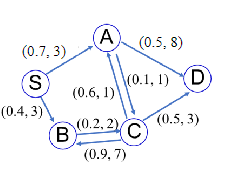
\includegraphics[scale=1]{HW4_Q3.png}
\begin{enumerate}
\item (a) Suppose the source node S wants to compute the shortest path from itself to all other nodes in the network. The shortest path is defined by hop count alone, without considering the cost and capacity of each link. Formulate the problem as a linear optimization problem.\\
\textbf{Answer:}Solve the problem in matrix format: $c^Tx$ subject to Ax = b\\
x = $[x_{SA}, x_{SB}, x_{AC}, x_{AD}, x_{BC}, x_{CB}, x_{CA}, x_{CD}]^T$\\
b = [S = 1 , A = 1, B = 0, C = 0, D = -2]\\
$A\:=\:\begin{pmatrix}1&1&0&0&0&0&0&0\\ -1&0&1&1&0&0&-1&0\\ 0&-1&0&0&1&-1&0&0\\ 0&0&-1&0&-1&1&1&1\\ 0&0&0&-1&0&0&0&-1\end{pmatrix}$\\

(b) Now take into account the cost of each link, and reformulate the optimization problem.\\
\textbf{Answer:}
x = $[x_{SA}, x_{SB}, x_{AC}, x_{AD}, x_{BC}, x_{CB}, x_{CA}, x_{CD}]^T$\\
b = [S = 1 , A = 1, B = 0, C = 0, D = -2]\\
$c = [0.7, 0.4, 0.1, 0.5, 0.2, 0.9, 0.6, 0.5]^T$\\
$A\:=\:\begin{pmatrix}1&1&0&0&0&0&0&0\\ -1&0&1&1&0&0&-1&0\\ 0&-1&0&0&1&-1&0&0\\ 0&0&-1&0&-1&1&1&1\\ 0&0&0&-1&0&0&0&-1\end{pmatrix}$\\

(c) Now there are two sets of source-destination pairs, S→D and B→D. All the links have cost 0, but limited capacity as indicated in the topology. Suppose a network operator wants to maximize the total throughput of these two source-destination pairs. Formulate the problem as an optimization problem\\
\textbf{Answer:} Then the objective is max $f_{S to D}$ + $f_{B to D}$ Subject to $0 <= x_{ij} <= u_{ij}$\\
x = $[x_{SA}, x_{SB}, x_{AC}, x_{AD}, x_{BC}, x_{CB}, x_{CA}, x_{CD}]^T$\\
b = [S = f , A = 0, B = f, C = 0, D = -2f]\\
u = $[3, 3, 1, 8, 2, 7, 1, 3]^T$\\
$A\:=\:\begin{pmatrix}1&1&0&0&0&0&0&0\\ -1&0&1&1&0&0&-1&0\\ 0&-1&0&0&1&-1&0&0\\ 0&0&-1&0&-1&1&1&1\\ 0&0&0&-1&0&0&0&-1\end{pmatrix}$\\

\end{enumerate}

%%%%%%%%% Q4
\noindent \textbf{Problem 4 (18pt). Wireless routing.\\}
\begin{enumerate}
\item (a) What are the main challenges for multi-hop routing in wireless networks, in comparison with multi-hop wireline networks?\\
\textbf{Answer:} Compared to multi-hop wireline networks, the main challenges are as follows:\\
High dynamic network topology: due to mobility\\
Highly dynamic link quality: due to channel condition changes\\
Cannot afford too frequent routing message exchange\\
Hop count no longer works
\item(b) Consider the following network topology. Link label $(x, y)$ indicates loss rate=x and link bit-rate=$y$ Mbps. Suppose links $A\rightarrow B$ and $D\rightarrow E$ can transmit concurrently, and any other pairs of links will interfere with each other if triggered simultaneously. Suppose A is the source node and E is the destination. What is the ETX metric for each link? What is the ETT metric? (You can ignore the ACK transmission time when calculating the ETT, as mentioned in the lecture). Suppose each data packet is 1 Kb. What is the optimal expected time to deliver 10 Mb of data? Is it equal to the sum of the expected time on each link? Explain how you derived the answers in detail.\\
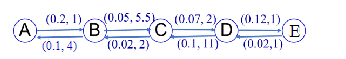
\includegraphics[scale = 1]{HW4_Q4.png}\\
\textbf{Answer:}\\
$Link\:ETX\:=\:\frac{1}{df\:\cdot \:dr}$, where\\
$ETT\left(b\right)\:=\:\frac{S}{b}\cdot ETX\left(b\right)$\\
df = forward link delivery ratio (data packet)\\
dr = reverse link delivery ratio (ack packet)\\
S = Packet Length\\
b = Transmission Rate\\
$A\rightarrow B$\\
ETX = $\frac{1}{(1-0.2)*(1-0.1)}$ = 1.389\\
ETT = $\frac{S}{1} * ETX $ = 1.389 S\\

$B\rightarrow C$\\
ETX = $\frac{1}{(1-0.05)*(1-0.02)}$ = 1.074\\
ETT = $\frac{S}{5.5} * ETX $ = 0.195 S\\

$C\rightarrow D$\\
ETX = $\frac{1}{(1-0.07)*(1-0.1)}$ = 1.195\\
ETT = $\frac{S}{2} * ETX $ = 0.597 S\\

$D\rightarrow E$\\
ETX = $\frac{1}{(1-0.12)*(1-0.02)}$ = 1.16\\
ETT = $\frac{S}{1} * ETX $ = 1.16 S\\

If S = 1Kb and $A\rightarrow B$ and $D\rightarrow E$ can transmit concurrently, the worst transmission rate dominates the transmission at that time slot.
Total = (1.389 + 0.195 + 0.597)Mbs * $\frac{1 Kb}{1 Mb}$ = 2.181 mSec\\
10 Mb = 2.181m * 10000 = 21.81 Sec\\
It is not equal to the sum of the expected time on each link (1.389 + 0.195 + 0.597 + 1.16 ) * 10 = 33.41 Sec. This is because there are two transmission occurring concurrently.
\end{enumerate}

%%%%%%%%% Q5
\noindent \textbf{Problem 5 (18pt). Wireless TCP.\\}
\begin{enumerate}
\item TCP doesn’t work well when an end-to-end path involves a wireless link. Why?\\
\textbf{Answer:} From the lecture 15. Generally, TCP interprets any packet loss as a sign of queue congestion. But for wireless links, packet loss can also be due to poor link quality. And. mobility also can lead to poor link quality. So the reducing window method in TCP lower the overall throughout.
\item What are the pros and cons of split TCP and Snoop TCP?\\
\textbf{Answer:} From the lecture 16\\
Split TCP:\\
Pros: No changes needed in wired network or content servers. Transmission faliure can be recovered locally.\\
Cons: Violation of end-toend design principle of the Internet (TCP becomes dependent on layer-2 devices and TCP no longer reliable if crash/bug at AP); Large buffer space may be needed at AP; AP must maintain per-TCP connection state; State must be forwarded to new AP on handoff.\\
Snoop TCP:\\
Pros: Alleviates most significant problem of split TCP; Downlink works without modification to mobile or server; Preserves end-to-end princip. Crash does not affect correctness, only performance.\\
Cons: The mobile host still needs to be modified at MAC and transport layers; the end-to-end principle is slightly violated.
\item How does an ELN access point (or basestation) determine whether an uplink packet loss is due to congestion or poor link condition? How does it notify the TCP sender about a link loss?\\
\textbf{Answer:} From lecture 16\\
The PHY later explicitly notifies TCP sender about the cause of packet loss.\\
In the ELN, AP keeps track of gaps(number of miss at seq xx) in the TCP packet received from the mobile sender. When AP sees a duplicate ACK, it compares with recorded gaps. If matches, AP sets the ELN bit in the duplicate ACK and forwards it. When mobile receives dup ack with ELN bit set, it resends the packet without reducing the congestion window.
\end{enumerate}

%%%%%%%%% Q6
\noindent \textbf{Problem 6 (14pt). Mobile applications.\\}
\begin{enumerate}
\item HTTP underutilizes the network capacity when running over a network path that contains a cellular link. What’s the reason behind?
\textbf{Answer:} From lecture 17\\
HTTP only generates a short, bursty flow; flow often ends before cwnd converges to true network capacity. And TCP works best only when there is a steady stream of data packets to drive the cwnd to converge to true capacity quickly. Moreover, this problem is even worse in wireless networks because wireless networks (cellular link) have longer RTT, which means lower throughput and a longer time for TCP to converge. Also, the mobility of wireless networks cause the network capacity to vary quickly.
\item Video applications encounter more performance issues when running over wireless networks? What’s the reason behind? What are the possible solutions? Why would they work?\\
\textbf{Answer:} From lecture 17\\
There is a continuous playout constraint to the video. However the network delays are not constant, so another client-side buffer is needed to match playout requirements. Moreover, video applications often involve lots of client interactivity, like pause, fast forward, rewinding, jumping through video, etc., so they need some buffer to store those video segments. Also, video packet loss happens over the wireless networks.\\
Solution 1: Smart buffering\\
The video receiver uses a larger buffer to smooth out the network capacity variation. But this only works for un-interactive video because interactive video needs lots of interactive actions. Also, the buffer size is hard to decide, as hard as choosing the optimal video bit rate itself.\\
Solution 2: Active bandwidth probing\\
The video server periodically sends some dummy data to estimate the network capacity and find the corresponding bit rate. But this solution costs extra network resources and needs to modify the video streaming application itself.\\
Solution 3: Physical layer informed mobile video streaming\\
Estime the wireless link capacity based on PHY layer statistics, like signal strength, time/frequency resource utilization, etc. The challenge is that it needs the wireless link to provide PHY later statistics.
\end{enumerate}
\end{document}